\chapter{Classification}
In this Chapter, the classification of the gathered data is been described. That means that the data is interpreted and put into a context which can be used to generate results in the next section.

\section{Context Classification}
In order to understand the gathered values from the sensors rather than just using them, it makes sense to interpret them and bring it into a context. Previous research results and also classifying controlled tested events using the gathered values will be described in further detail within the next paragraphs.

\subsubsection{Indoor Outdoor differentiation}
The brightness of indoor lightning is different from the brightness outdoors. Indoor environments are mostly receiving light from an artificial light source which flickers in a rate than can't be noticed by the human eye. Sadly the light sensor of the mobile devices is not precise enough to detect that flickering. Anyhow, also the luminance is different indoors and outdoors. Indoor lights are just not as powerful as the sun and it would require a ridiculous amount of artificial light sources and windows to create the same brightness within buildings as they are outside. 
As seen in the two tables \ref{outLight} and \ref{inLight}, based on the lux from the light sensor it is possible to give an educated guess whether the mobile device is indoor or outdoor.

%%%% TABLE outdoor light
\setlength{\tabcolsep}{10pt}
\renewcommand{\arraystretch}{1.5}
{\rowcolors{3}{black!10!white!90}{white!100}

\begin{table}[!htb]
\centering
\begin{tabular}{ |p{4cm}|p{4cm}|  }
 \hline
 \rowcolor{lightgray} \multicolumn{2}{|c|}{{\bf Common Light Levels Outdoor - Daytime}} \\
 \hline
{\bf Condition} & {\bf Illumination in lux}\\
 \hline
 Sunlight   		& 107,527\\
 Full Daylight   	& 10,752.7\\
 Overcast Day	& 1,075.3\\
 Very Dark Day	& 107,527\\
 \hline
\end{tabular}
\caption{Common Outdoor Light Levels}
\label{outLight}
\end{table}

%%%% TABLE indoor light
\begin{table}[!htb]
\centering
\begin{tabular}{ |p{10cm}|p{4cm}|  }
 \hline
 \rowcolor{lightgray} \multicolumn{2}{|c|}{{\bf Common and Recommended Light Levels Indoor}} \\
 \hline
{\bf Activity/Location} & {\bf Illumination in lux}\\
 \hline
 Warehouses, Homes, Theaters, Archives   																	& 150\\
 Easy Office Work, Classes   																						& 250\\
 Normal Office Work, PC Work, Study Library, Groceries, Show Rooms, Laboratories	& 500\\
 Supermarkets, Mechanical Workshops, Office Landscapes 											& 750\\
 Normal Drawing Work, Detailed Mechanical Workshops, Operation Theatres 				& 1,000\\
 Detailed Drawing Work, Very Detailed Mechanical Works 											& 1,500 - 2,000\\
 \hline
\end{tabular}
\caption{Common \& Recommended Indoor Light Levels}
\label{inLight}
\end{table}

\FloatBarrier
\clearpage

\subsubsection{Movement of Mobile Phone}
The Y and Z axis of the 3D accelerometer can be used to detect whether the participant moves and uses the mobile phone.\\
The values from the 3 axis can give an indicator how the participant interacts with the device. For the results, we want to know, how many times user picks up the mobile phone and how long he/she was interacting with it. That behavior, as shown in the graphic \ref{accDev} detects changes between the mobile device laying flat on the desk and the device being in a vertical position by the changes in the rotation of the z- and y-axis.  

\begin{figure}[!htb]
\centering
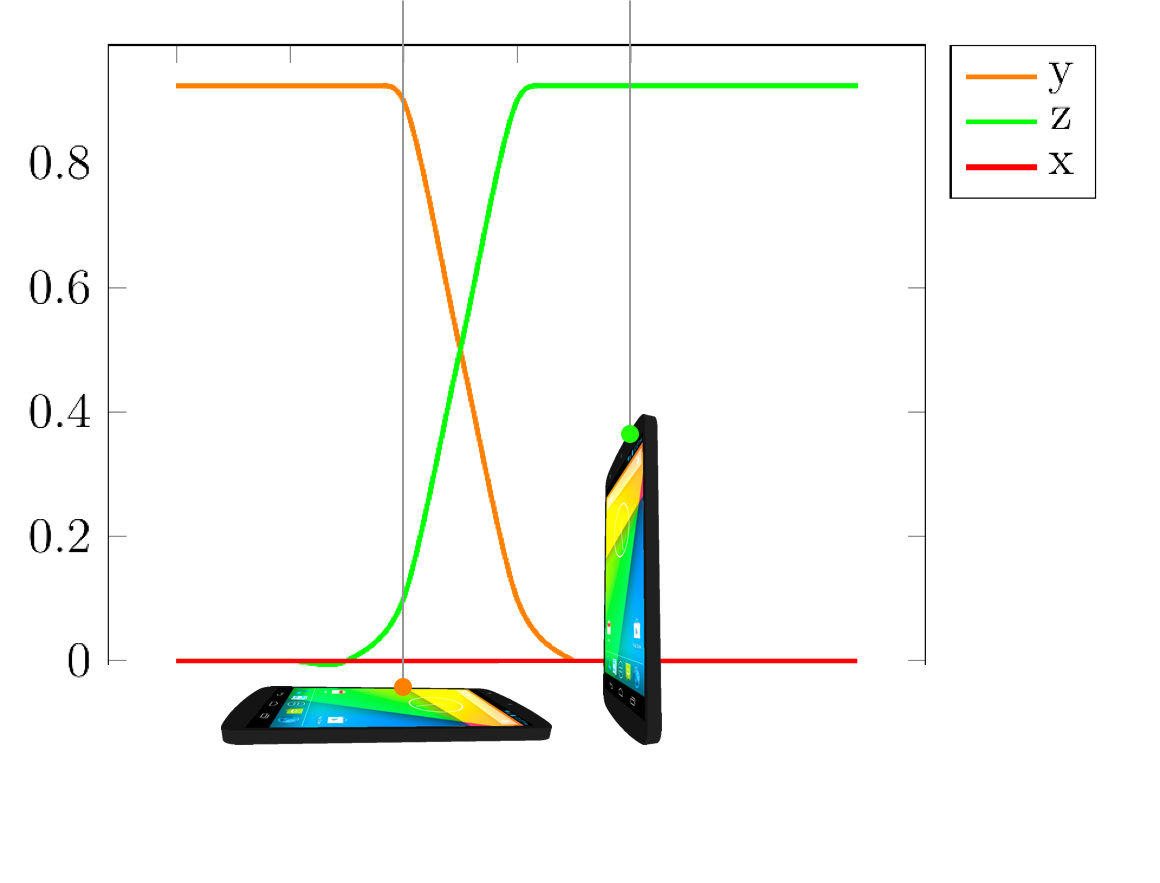
\includegraphics[width=10cm]{accDevice}
\caption{Device Rotation}\label{accDev}
\vspace{10 mm}
\end{figure}
\FloatBarrier

\subsubsection{Location}
In order to detect the location of the user, the location with the environmental noise as well as the detection whether the user is indoor our outside. The location accuracy depends on the way how it is been calculated which is ether the network or GPS. However, it can vary and can't ensure a the exact location but also using the noise and information from the light sensor can help to limit the results to fewer possibilities.\\
When, for example the location shows a radius in an area with a library, a coffee shop and a public crowded square it's a high chance that the library is not an option in the case of a noisy environment. In order to detect whether the user is in the coffee-shop or the square, the light sensor can detect whether the light value is in the outdoor or indoor brightness range. 

\subsubsection{Movement}
The movement of the user can directly be seen by the steps he/she walks during the start of the gathering until the ending. The distance and the frequency shows if the user just walks to the fridge, toilet or somewhere close or actually walks from one place to another. Also the locations can indicate that.\\
The location can also show whether the user was on public transport, on a train/car or an Airplane depending on the travel speed and from where the user started and where he/she arrives (airport, garage, train-station etc.). 

\subsubsection{Weather Conditions}
With the location and the timestamp of the gathering and it is possible to get information about the local weather of the users location at the time when the gathering happened using the timeanddate-website \footnote{\url{http://www.timeanddate.com/weather}}.


\subsubsection{Dynamic}
The dynamic in values is the way it differentiates in itself. This information can be used to detect changes in the noise level and environmental light. For detecting a range within the dataset a range must be set which value are within a normal range and which are falling out. One way to calculate a range is to use the standard deviation + and - to the mean of the values. 

\subsubsection{Music}
Using the environmental noise it is possible to find patterns that can be related to music. In general modern music has a very constant noise level rather than the dynamic classical music. The iTunes top 100\footnote{\url{http://www.apple.com/ie/itunes/charts}} songs at July 14th 2016 have an average length of 3:39 minutes, the shortest song is 2:42 minutes and the longest 5:13 minutes long.\\
In order to detect whether the participant is listening to music, the volume should go down for 2-5 seconds between a track with a duration between 2:30 minutes and 5:30 minutes. 
A regular pattern with these attributes should indicate that the user is listening to background music while working on the coding task.

\subsection{Questions}
After the gathering process, the participant was asked to answer some questions:
\begin{itemize}
\item Are you a Student?
\item Did you work in a team?
\item Did you listen to music?
\item Did you feel tired?
\item Did you enjoy the tasks?
\item Did you give all you attention to the tasks?
\item Were you distracted during the tasks?
\item Did you feel stressed
\item Do you think the tasks were easy?
\end{itemize}

All the questions can either be checked to indicate 'yes' or leave unchecked for 'no'. The answers can help to clarify the classification or to get new additional contexts. Some of the questions are created based on the knowledge from previous work of researchers and their results that can possibly influence cognitive performance. \\
In a long term, asking questions is not optimal. In the future the app is supposed to learn and slowly make the questions unnecessary. Currently there is a way to detect whether the user is listening to music by identifying patterns but the accuracy is not exactly known and therefore also asked as a question as well could it be that the user is wearing headphones. If the detection using the environmental noise is highly accurate, the question can be removed from the app.